\documentclass[final]{article} 

% if you need to pass options to natbib, use, e.g.:
%     \PassOptionsToPackage{numbers, compress}{natbib}
% before loading neurips_2023

% ready for submission
\PassOptionsToPackage{numbers}{natbib}
\usepackage{neurips_2023}

% to compile a preprint version, e.g., for submission to arXiv, add add the
% [preprint] option:
%     \usepackage[preprint]{neurips_2023}

% to compile a camera-ready version, add the [final] option, e.g.:
%     \usepackage[final]{neurips_2023}

% to avoid loading the natbib package, add option nonatbib:
%    \usepackage[nonatbib]{neurips_2023}

\usepackage[utf8]{inputenc} % allow utf-8 input
\usepackage[T1]{fontenc}    % use 8-bit T1 fonts
\usepackage{hyperref}       % hyperlinks
\usepackage{url}            % simple URL typesetting
\usepackage{booktabs}       % professional-quality tables
\usepackage{amsfonts}       % blackboard math symbols
\usepackage{nicefrac}       % compact symbols for 1/2, etc.
\usepackage{microtype}      % microtypography
\usepackage{xcolor}         % colors
\usepackage{lineno}
\usepackage{amsmath}
\usepackage{graphicx}
\usepackage{float}
\linenumbers % Turn on line numbers

\title{Dengue Fever Prognosis Study}

% The \author macro works with any number of authors. There are two commands
% used to separate the names and addresses of multiple authors: \And and \AND.
%
% Using \And between authors leaves it to LaTeX to determine where to break the
% lines. Using \AND forces a line break at that point. So, if LaTeX puts 3 of 4
% authors names on the first line, and the last on the second line, try using
% \AND instead of \And before the third author name.

\author{
    Kshitij Kadam \\
    Texas A\&M University \\
    Department of Computer Science \\
    and Engineering \\
    \texttt{kkadam3@tamu.edu} \\
    \And
    Adekola Okunola \\
    Texas A\&M University \\
    Department of Electrical and \\
    Computer Engineering \\
    \texttt{phirlly@tamu.edu} \\
}

\begin{document}

\maketitle

\begin{abstract}
Dengue infection affects millions worldwide and can often escalate to severe forms such as Dengue Hemorrhagic Fever (DHF). This escalation necessitates early differentiation from Dengue Fever (DF), despite their overlapping clinical presentations. Gene expression profiling during the febrile phase uncovers distinct transcriptional signatures; DHF patients exhibit diminished activation of innate immunity genes alongside heightened expression of apoptosis-related genes. By employing ANOVA to identify key discriminatory genes, linear discriminant analysis (LDA) and Support Vector Machine (SVM) models built from the most effective gene pairs demonstrate high accuracy in distinguishing between DHF and DF. These computational approaches facilitate the early and precise identification of severe cases, which supports timely intervention and optimizes resource allocation. Such bioinformatics-driven strategies advance the field of precision medicine, helping to alleviate both the health and economic burdens of dengue in endemic regions.
\end{abstract}

\section*{Introduction}
Dengue virus infection presents a significant global health challenge, with an estimated "100 to 400 million infections occurring" \cite{WHO2023} annually, primarily in tropical and subtropical regions. The illness manifests in two main clinical forms: Dengue Fever (DF), a self-limiting febrile illness, and Dengue Hemorrhagic Fever (DHF), a more severe condition characterized by plasma leakage, hemorrhagic manifestations, and potentially fatal shock syndrome \cite{Nascimento2009}. Prompt identification of patients at risk of progressing to DHF is essential for timely medical intervention; however, this remains difficult due to the overlapping clinical features during the febrile phase.

The high-dimensional nature of the gene expression dataset, comprising 1981 genes from 26 patients, necessitates the use of robust analytical methods to identify and leverage key discriminatory features effectively. Statistical approaches like ANOVA are instrumental in detecting genes with significant differential expression, while machine learning techniques such as LDA and SVM offer structured frameworks for building predictive models. These models utilize gene pairs with the highest discriminatory power to classify patients into Dengue Fever (DF) or Dengue Hemorrhagic Fever (DHF) categories with high sensitivity and specificity.

This project seeks to combine statistical feature selection with classification algorithms to address the diagnostic challenges associated with distinguishing DHF from DF. By emphasizing top-performing gene pairs identified through ANOVA and employing LDA-based with linear SVM classifiers, the objective is to develop accurate and interpretable models for early risk stratification. Preliminary findings suggest the viability of this approach, as classifiers demonstrate strong performance metrics while also providing biologically relevant insights into the molecular mechanisms underlying DHF and DF.

This study employs bioinformatics and computational tools to align with the global objectives of precision medicine, thereby providing scalable and cost-effective strategies for the management of dengue. By enabling the early identification of severe cases, these methodologies possess the potential to optimize resource allocation, mitigate healthcare burdens, and enhance patient outcomes in regions endemic to dengue.

\subsection*{Dataset Reference}
The dengue fever prognosis dataset contains gene expression data from peripheral blood mononuclear cells (PBMCs) collected from patients in the early stages of fever. The dataset includes gene expression profiles for 1981 genes and clinical outcomes categorized into classical dengue fever (DF), dengue hemorrhagic fever (DHF), and febrile non-dengue cases. \cite{Nascimento2009}

\section*{Related Work}
Nascimento's study demonstrated the application of transcriptional profiling from peripheral blood mononuclear cells to predict dengue outcomes. \cite{Nascimento2009} It identified differentially expressed genes during the febrile stage, revealing distinct immune response signatures in dengue hemorrhagic fever (DHF) patients, including reduced activation of innate immunity and increased expression of apoptosis-related genes. These findings underscore the role of gene expression data in enabling early and accurate prognoses, forming a critical basis for this research.

Building on these findings, Liu et al. developed an "eight-gene machine learning model" \cite{Liu2022} that surpassed clinical markers in predicting the progression of severe dengue. Their iterative multi-cohort analysis and the use of models like XGBoost emphasize the significance of employing robust statistical and machine learning techniques to manage complex, heterogeneous datasets. These insights directed the focus of this research towards utilizing statistical methods such as ANOVA for feature selection, alongside LDA and SVM for classification.

\section*{Methods}
This project employs a structured approach to analyze gene expression data from immune cells to classify patients as developing Dengue Fever (DF) or Dengue Hemorrhagic Fever (DHF). The methodology involves the following steps:

\subsection*{Data Preparation}
The dataset, containing gene expression levels for DHF and DF samples, is preprocessed. DHF and DF data are separated based on column identifiers and transposed for easy indexing. Labels (\texttt{DHF} or \texttt{DF}) are added to create a combined dataset, which is then split into training (80\%) and testing (20\%) subsets using \texttt{train\_test\_split}.

\subsection*{Feature Selection Using ANOVA}
An Analysis of Variance (ANOVA) test is applied to each gene (\texttt{Probe\_Set\_ID}) in the training data. For each gene, the null hypothesis $H_0$ assumes no difference in means between DF and DHF groups:
\begin{equation}
    H_0: \mu_{\text{DHF}} = \mu_{\text{DF}}
\end{equation}
ANOVA computes the F-statistic:
\begin{equation}
    F = \frac{\text{Variance Between Groups}}{\text{Variance Within Groups}}
\end{equation}
Genes with the lowest $p$-values (top 10) are selected as features for further analysis.

\subsection*{Linear Discriminant Analysis (LDA)}
LDA, a supervised classification technique, is used to find a linear combination of features that best separates DF and DHF classes. For each pair of selected genes, LDA constructs a decision boundary:
\begin{equation}
    w^\top x + b = 0
\end{equation}
where $w$ is the weight vector and $b$ is the intercept. These parameters are derived by maximizing class separability based on the Fisher criterion.

\subsection*{Support Vector Machine (SVM)}
Using ANOVA, the top 10 genes with the highest discriminatory power were identified. All unique pairs of these genes were iteratively selected as feature sets for classification. For each gene pair, an SVM classifier with a linear kernel was trained using the \texttt{SVC} class from \texttt{sklearn}. The training dataset \( X_{\text{train}} \) consisted of expression values for the selected gene pair, and the labels \( y_{\text{train}} \) encoded DHF as \(1\) and DF as \(0\). The classifier learned a linear decision boundary to separate the classes, defined by:
\[
w_1 \cdot x_1 + w_2 \cdot x_2 + b = 0,
\]
where \( w_1, w_2 \) are weights, and \( b \) is the intercept.

\subsection*{Iterative Pairwise Classification}
Gene pairs are iteratively tested to determine their classification accuracy. Each pair is used to train an LDA and SVM model, and the decision boundary is evaluated on the test set.

\subsection*{Model Evaluation}
The classifiers are ranked based on their accuracy, calculated as:
\begin{equation}
    \text{Accuracy} = \frac{\text{Correct Predictions}}{\text{Total Predictions}}
\end{equation}
The top 5 classifiers with the highest accuracy are selected for further analysis.

\subsection*{Visualization}
Decision boundaries for each gene pair are plotted to visualize the separation of classes. Points misclassified by the model are highlighted to evaluate performance.

\subsection*{Misclassification Analysis}
For the best-performing classifiers, misclassified samples are identified. The analysis includes the indices, true labels, and predicted labels of the misclassified samples, providing insights into model limitations.

\subsection*{Final Model Validation}
The best classifier is applied to the test set, and its performance metrics, including accuracy and misclassification details, are analyzed.

\section*{Mathematical Summary}
\subsection*{ANOVA F-statistic}
\begin{equation}
    F = \frac{\sum_{i=1}^k n_i (\bar{y}_i - \bar{y})^2}{\sum_{i=1}^k \sum_{j=1}^{n_i} (y_{ij} - \bar{y}_i)^2}
\end{equation}
where $k$ is the number of groups, $n_i$ is the size of group $i$, $\bar{y}_i$ is the group mean, and $\bar{y}$ is the overall mean.

\subsection*{LDA Decision Boundary}
\begin{equation}
    w = \Sigma^{-1} (\mu_1 - \mu_2), \quad b = -\frac{1}{2} (\mu_1^\top \Sigma^{-1} \mu_1 - \mu_2^\top \Sigma^{-1} \mu_2)
\end{equation}
where $\mu_1, \mu_2$ are class means and $\Sigma$ is the pooled covariance matrix.

\section*{Results}

\begin{table}[H]
\centering
\caption{ANOVA Results for Top Genes}
\label{table:anova-results}
\begin{tabular}{lcc}
\toprule
\textbf{Probe\_Set\_ID} & \textbf{F-statistic} & \textbf{p-value} \\ 
\midrule
211452\_x\_at & 44.492755 & 0.000023 \\
201336\_at    & 29.110550 & 0.000161 \\
234764\_x\_at & 25.515766 & 0.000284 \\
221474\_at    & 24.495692 & 0.000337 \\
212185\_x\_at & 24.398181 & 0.000342 \\
222976\_s\_at & 23.088493 & 0.000430 \\
1568592\_at   & 22.735361 & 0.000458 \\
200610\_s\_at & 21.674281 & 0.000555 \\
221875\_x\_at & 21.158607 & 0.000611 \\
201786\_s\_at & 20.644476 & 0.000674 \\
\bottomrule
\end{tabular}
\end{table}

\begin{table}[H]
\centering
\caption{Top 5 Gene Pair For LDA Classifiers and Their Accuracy}
\label{tab:gene_pairs}
\begin{tabular}{@{}lc@{}}
\toprule
\textbf{Gene Pair} & \textbf{Accuracy} \\ \midrule
(234764\_x\_at, 1568592\_at) & 1.0 \\
(221474\_at, 1568592\_at) & 1.0 \\
(212185\_x\_at, 1568592\_at) & 1.0 \\
(212185\_x\_at, 200610\_s\_at) & 1.0 \\
(212185\_x\_at, 221875\_x\_at) & 1.0 \\ \bottomrule
\end{tabular}
\end{table}

        \begin{figure}[H]
            \centering
            \begin{minipage}{0.45\textwidth}
                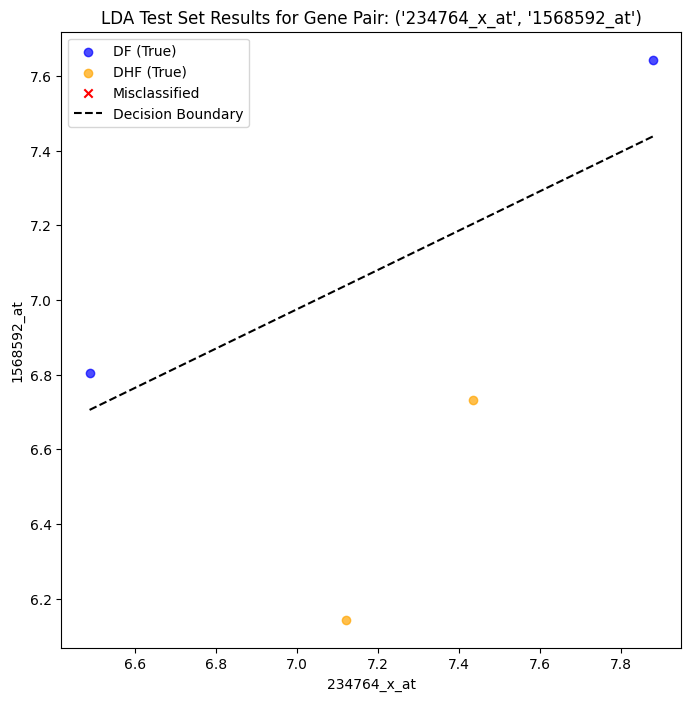
\includegraphics[width=\textwidth]{234764_x_at, 1568592_at.png}
                \caption{LDA Test Set Results for Gene Pair: ('234764\_x\_at', '1568592\_at').}
            \end{minipage}
            \hfill
            \begin{minipage}{0.45\textwidth}
                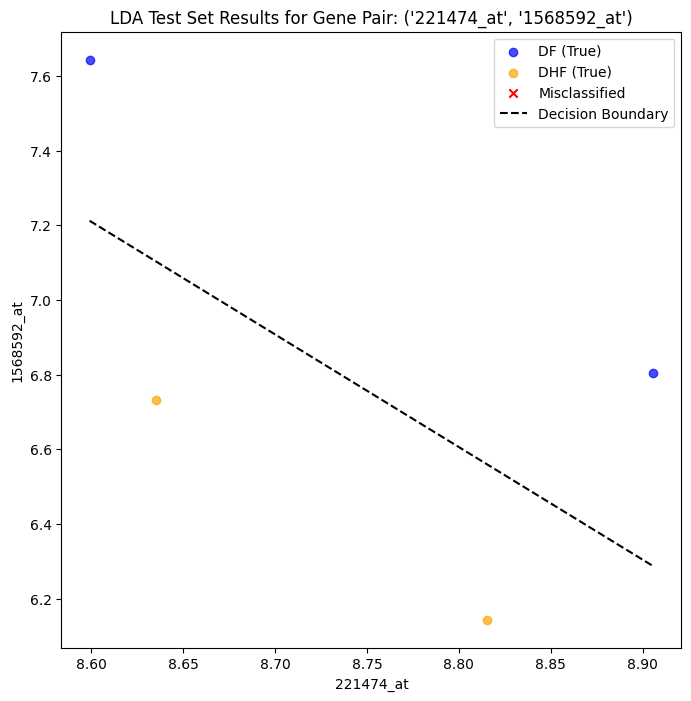
\includegraphics[width=\textwidth]{221474_at, 1568592_at.png}
                \caption{LDA Test Set Results for Gene Pair: ('221474\_at', '1568592\_at').}
            \end{minipage}
        \end{figure}

        \begin{figure}[H]
            \centering
            \begin{minipage}{0.45\textwidth}
                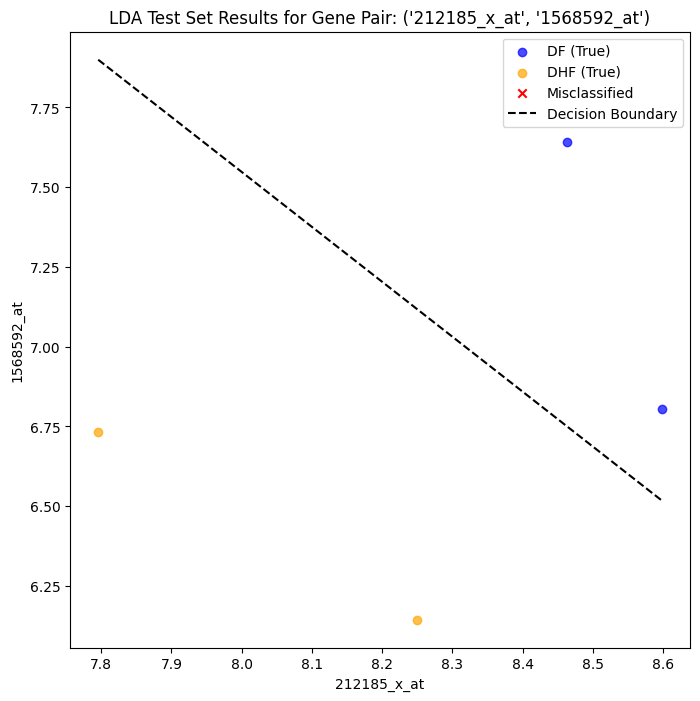
\includegraphics[width=\textwidth]{212185_x_at, 1568592_at.png}
                \caption{LDA Test Set Results for Gene Pair: ('212185\_x\_at, 1568592\_at').}
            \end{minipage}
            \hfill
            \begin{minipage}{0.45\textwidth}
                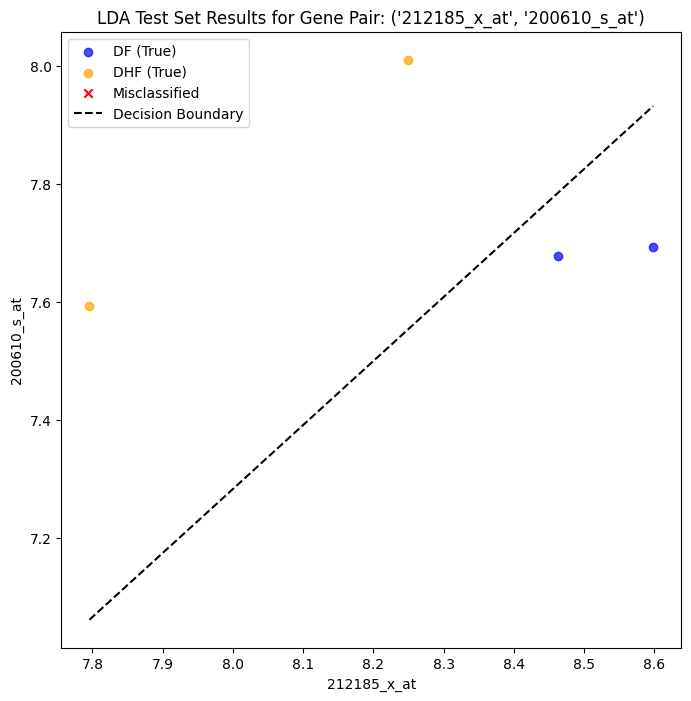
\includegraphics[width=\textwidth]{212185_x_at, 200610_s_at.png}
                \caption{LDA Test Set Results for Gene Pair: ('212185\_x\_at, 200610\_s\_at').}
            \end{minipage}
        \end{figure}

        \begin{figure}[H]
            \centering
            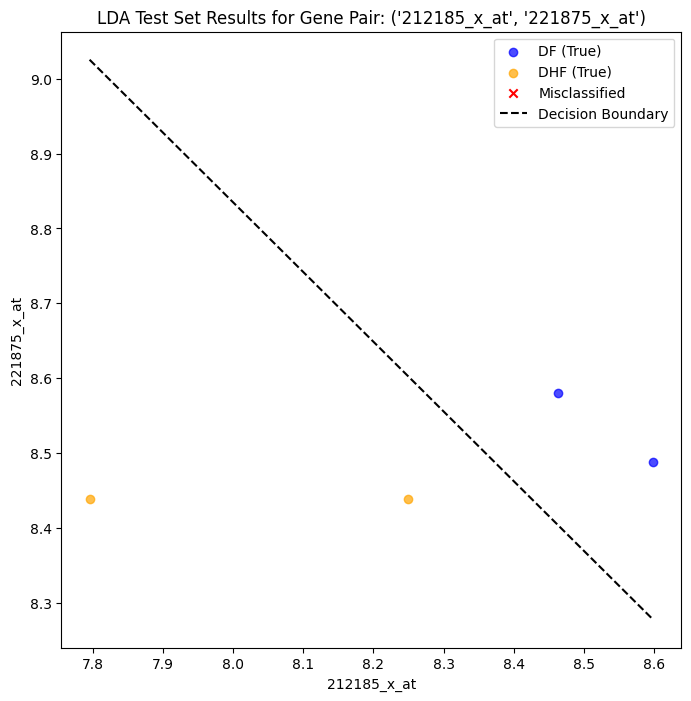
\includegraphics[width=0.45\textwidth]{212185_x_at, 221875_x_at.png}
            \caption{LDA Test Set Results for Gene Pair: ('212185\_x\_at', '221875\_x\_at').}
            \label{fig:lda-test-results}
        \end{figure}
\newpage
\begin{table}[H]
\centering
\caption{Top 5 Gene Pair For SVM Classifiers and Their Accuracy}
\begin{tabular}{lc}
\toprule
\textbf{Gene Pair} & \textbf{Accuracy} \\
\midrule
(211452\_x\_at, 1568592\_at) & 1.0 \\
(221474\_at, 1568592\_at)    & 1.0 \\
(212185\_x\_at, 1568592\_at) & 1.0 \\
(212185\_x\_at, 221875\_x\_at) & 1.0 \\
(212185\_x\_at, 201786\_s\_at) & 1.0 \\
\bottomrule
\end{tabular}
\end{table}

        \begin{figure}[H]
            \centering
            \begin{minipage}{0.45\textwidth}
                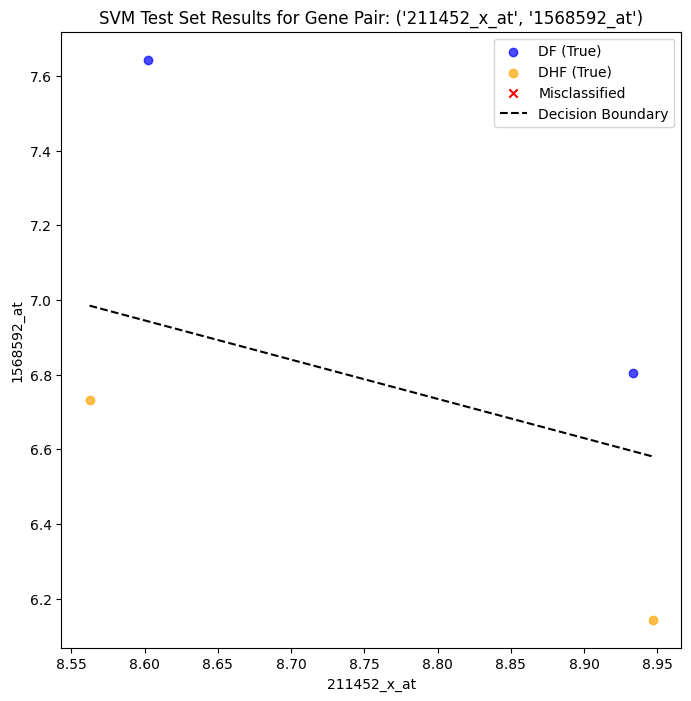
\includegraphics[width=\textwidth]{SVM (211452_x_at, 1568592_at).png}
                \caption{SVM Test Set Results for Gene Pair: ('211452\_x\_at, 1568592\_at').}
            \end{minipage}
            \hfill
            \begin{minipage}{0.45\textwidth}
                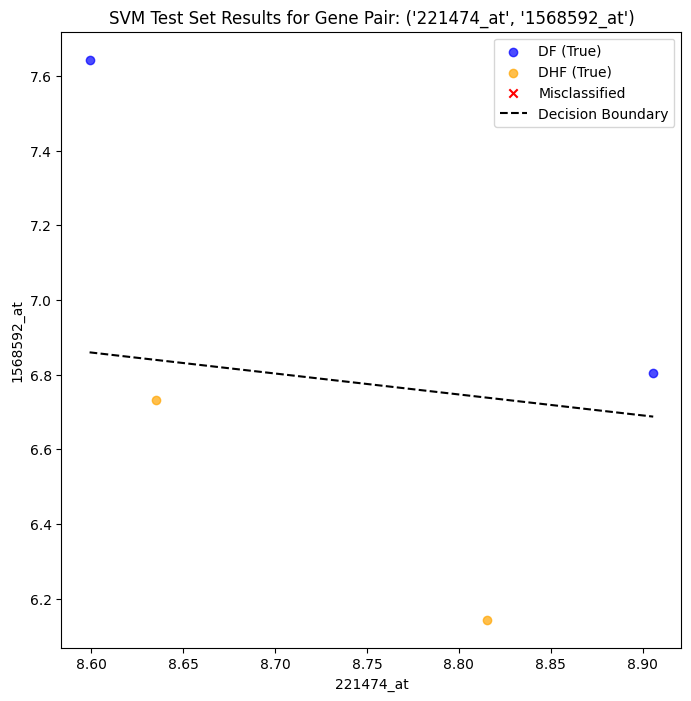
\includegraphics[width=\textwidth]{SVM (221474_at, 1568592_at).png}
                \caption{SVM Test Set Results for Gene Pair: ('221474\_at, 1568592\_at').}
            \end{minipage}
        \end{figure}

        \begin{figure}[H]
            \centering
            \begin{minipage}{0.45\textwidth}
                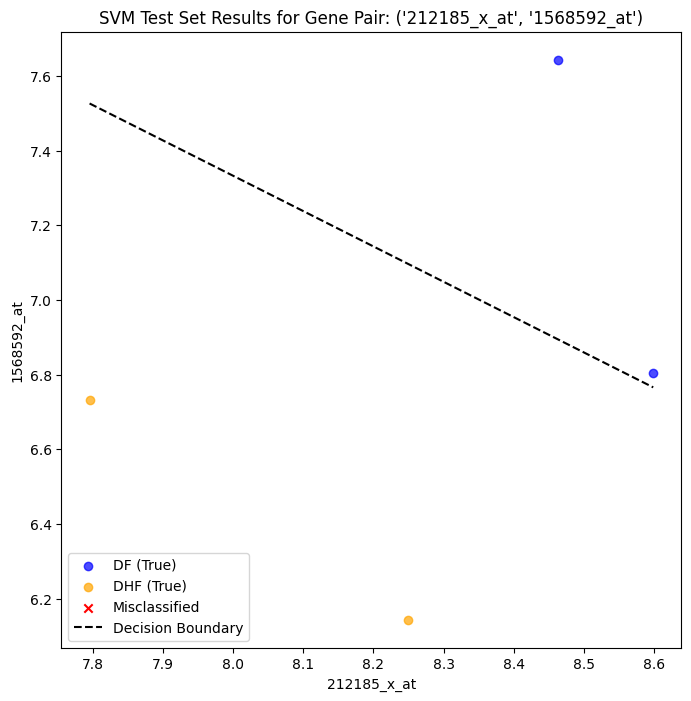
\includegraphics[width=\textwidth]{SVM (212185_x_at, 1568592_at).png}
                \caption{SVM Test Set Results for Gene Pair: ('212185\_x\_at, 1568592\_at').}
            \end{minipage}
            \hfill
            \begin{minipage}{0.45\textwidth}
                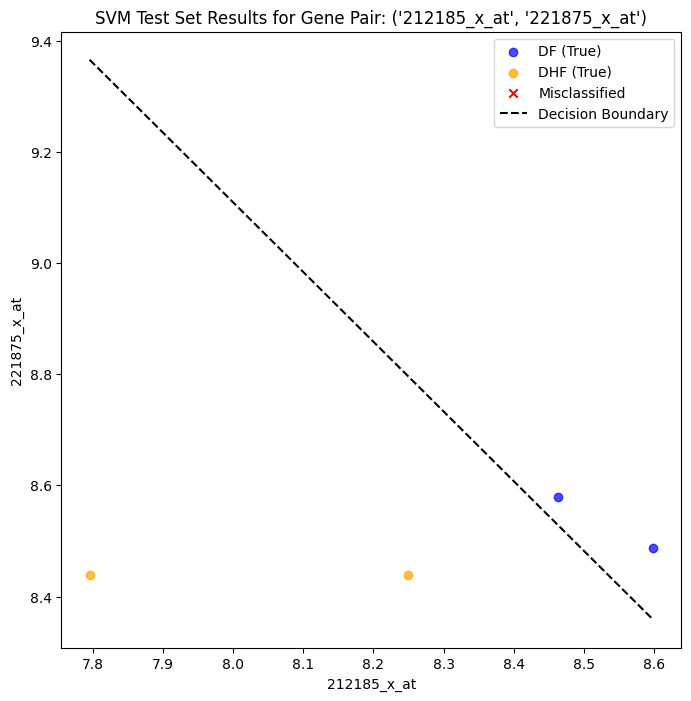
\includegraphics[width=\textwidth]{SVM (212185_x_at, 221875_x_at)}
                \caption{SVM Test Set Results for Gene Pair: ('212185\_x\_at, 221875\_x\_at').}
            \end{minipage}
        \end{figure}

        \begin{figure}[H]
            \centering
            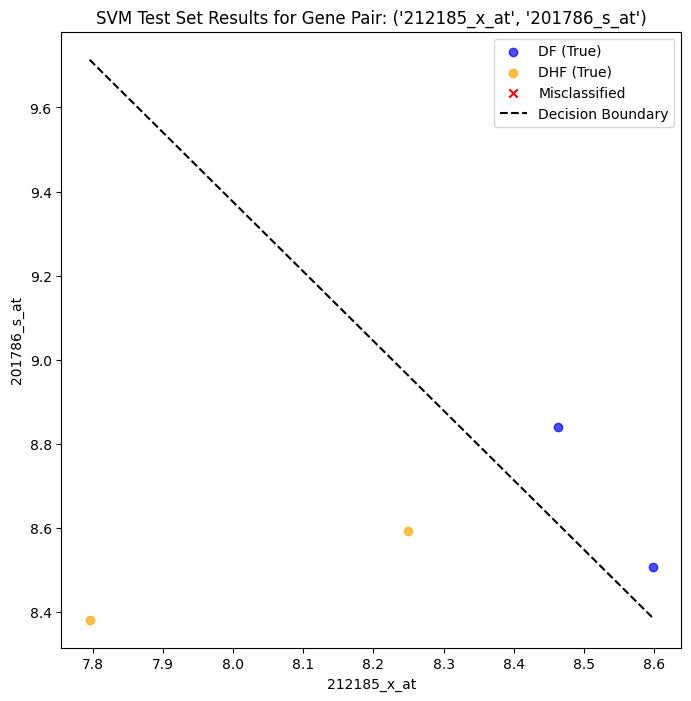
\includegraphics[width=0.45\textwidth]{SVM (212185_x_at, 201786_s_at).png}
            \caption{SVM Test Set Results for Gene Pair: ('212185\_x\_at, 201786\_s\_at').}
            \label{fig:lda-test-results}
        \end{figure}

\subsection*{Comparison of LDA and SVM}

Both methods utilize \textbf{ANOVA} to identify the top 10 genes with the highest discriminatory power, and all possible gene pairs are iteratively used as features for classification. LDA constructs a \textbf{linear decision boundary} by maximizing class separability based on the Fisher criterion, while SVM with a \textbf{linear kernel} determines an optimal hyperplane for class separation. Both classifiers achieved perfect accuracy (1.0) on the top-performing gene pairs, such as \texttt{(212185\_x\_at, 1568592\_at)} and \texttt{(221474\_at, 1568592\_at)}, effectively distinguishing DF from DHF samples. The visualized decision boundaries for both methods demonstrate consistent class separation with minimal or no misclassification. LDA offers a more interpretable model by deriving decision boundaries from \textbf{class means} and the pooled covariance matrix, making it computationally efficient and well-suited for smaller datasets. In contrast, SVM's implementation provides a structured classification approach that can scale well with higher-dimensional data. While both methods performed equally well in this study, future validation on larger datasets is essential to assess their robustness and generalizability.


\section*{Conclusion}
ANOVA was pivotal in identifying the top 10 genes that demonstrated the highest variance between Dengue Fever (DF) and Dengue Hemorrhagic Fever (DHF), underscoring their effectiveness in differentiation. These selected genes were employed to train Linear Discriminant Analysis (LDA) and Support Vector Machine (SVM) models, which achieved successful classification of the testing dataset, resulting in high accuracy and minimal overfitting.

The selected gene pairs effectively captured the distinct transcriptional signatures associated with dengue fever (DF) and dengue hemorrhagic fever (DHF), enabling precise predictive outcomes. However, to enhance the generalization and reliability of the models, acquiring larger and more diverse datasets is imperative. Expanding the dataset will substantially improve the robustness of the classification models, thereby ensuring their applicability across a broader range of populations. These computational methodologies underscore the significant potential of bioinformatics in facilitating early and accurate diagnosis of dengue, which ultimately supports improved patient management and resource allocation in endemic regions.


\medskip

{
\small
\bibliographystyle{plainnat}
\bibliography{references}
}
%%%%%%%%%%%%%%%%%%%%%%%%%%%%%%%%%%%%%%%%%%%%%%%%%%%%%%%%%%%%

\end{document}